\def\DevnagVersion{2.15}\documentclass[a4paper, 10pt, notitlepage]{report}

\usepackage{amsfonts} % if you want blackboard bold symbols e.g. for real numbers
\usepackage{graphicx} % if you want to include jpeg or pdf pictures
\usepackage{devanagari}
\usepackage{xcolor}
\usepackage{geometry}
\geometry{
    body={6.0in,9.5in},
    left= 1.0in,
    top = 0.5in}

\usepackage{hyperref}
\hypersetup{
    colorlinks,
    citecolor=black,
    filecolor=black,
    linkcolor=blue,
    urlcolor=black
}
\usepackage{color}
\definecolor{gray1}{RGB}{192,192,192}
\definecolor{gray}{RGB}{240,240,240}
%\title{Action Discovery in Psychological Videos and Hindi Verb Modelling} % change this
\author{Diwakar Chauhan} % change this
\date{\today} % change this

\begin{document}
\begin{center}
%\renewcommand{\rmdefault}{ptm}

{\color{blue} \fontfamily{rmdefault} \textsc{\LARGE IIT Kanpur}\\[1.5cm] }
\textsc{\Large B.Tech Project}\\[1cm]
\hrule height 2pt
\vspace*{10pt}
%\end{center}
{\huge  Action Discovery in Psychological Videos and Hindi Verb Modelling}\\[0.4cm] 
\hrule height 2pt 
\vspace*{10pt}
%\\[1cm]
\begin{minipage}{0.4\textwidth}
\begin{flushleft} \large
\emph{Author:}\\
{\color{blue} \href{http://home.iitk.ac.in/~diwakarc}{Diwakar Chauhan} }
\end{flushleft}
\end{minipage}
\begin{minipage}{0.4\textwidth}
\begin{flushright} \large
\emph{Supervisor:} \\
{\color{blue} \href{http://www.cse.iitk.ac.in/users/amit}{Prof. Amit Mukerjee } }% Supervisor name - remove the \href bracket to remove the link  
\end{flushright}
\end{minipage}\\[3cm]


{\large \today}\\[4cm] % Date
%%%%%%%%%% PRELIMINARY MATERIAL %%%%%%%%%%
%\maketitle
%\begin{center}
%Supervised by Dr. Amit Mukerjee % change this
\end{center}

\thispagestyle{empty}

\newpage
\section*{Acknowledgements} % this must be included in undergradate projects
I am very thankful to people who have helped me with this project directly or indirectly.
Many-many thanks to Dr. Uta Frith, Institute of Cognitive Neuroscience,University College London, and  her Ph.D student Sarah White for providing me with psychological videos.\\%acknowledgement for utah Frith
%Sushobhan Nayak
%Prashant Jalan

\tableofcontents 

\newpage
%%%%%%%%%% MAIN TEXT STARTS HERE %%%%%%%%%%
\section*{Abstract}
{\it
Human learning process involves learning the identity of objects(nouns) the relationship between the object(preposition) and the interaction of objects. An infant learns the identities of objects in first place than verbs. The reason behind this may be that verbs therefore activities, require more information. Naigles(1990)\cite{naigles} demonstrated that while learning meaning of verbs, infants use the syntactic information. She proved that given a illegal verbs in a sentence the children use the syntax to guess the meaning of the verb. \\
\hspace*{10pt} However difficult the learning process of infants may be, they do not analyse large amount of data in order to learn the meanings of verbs or recognize the activities. They learn from the competent speakers who know relate the words to the event's objects in the environment.\cite{kerr-cohen-08_wubble-world-lang-acquisition} And the children can extend their learning from one event to another. 
\hspace*{10pt} Here we are trying to understand the leaning process of infant and based on that learning process, try to discover actions in psychological videos and map Hindi verbs to them.
}

%%%%%%%%%% SAMPLE CHAPTER %%%%%%%%%%
\chapter{Introduction}
\hrule height 2pt
\vspace*{10pt} 
 Actions can be based on the the variations in the shape and size change , poses\cite{pami-Ben-ArieWPR02}  or orientation of the object. For example a person walking can be identified by motion of his hands and legs relative to his body. Similar can be said about the actions involving multiple agents. But what if the action which either don't need any shape changes to be expressed or the agent is an abstract object. These type of actions are represented either by specific motion of single object or particular type of motions and interaction between the agents. In this project we analyse the second type of actions. We use psychological videos\cite{fhanimation}. \\

%%place samples from the video
\hspace*{10pt} Most of these animations contain only two agents which are triangles. The videos represent a particular transitive action.The videos,each of them represents certain action either complex or simple. By complex action we mean that the action constitutes smaller actions, e.g. the "Coxing" in the video consists of many instances of "Pushing" and "Rotating Jointly". We take some of the videos and apply HMM to on the feature vectors extracted from the frames of video. We take frames in small consecutive groups. We create HMM for each of this groups and evaluate the mutual acceptance measure for each of the groups. Based on this measure, hierarchical clustering is created. This cluster tree is later cut at some point to produce certain number of clusters.
\hspace*{10pt} At the same time commentary is taken for the video. This commentary is processed to remove less important words and association measures are calculated for each of the remaining words. Based on this association measure, the nouns are identified.

\paragraph{Unnumbered paragraph heading}
The text of this paragraph.

\chapter{Prelinguistic Image Schemata}
%\vspace*{5pt}
\hrule height 2pt
\vspace*{10pt}
Before mapping the language to visual sequences, we need to get the properties of the visual sequences.\\
\section{Agents in the visual sequences}
A sentence in a language consists of small units of words, phrases appearing as different parts of speech for that language. Theses different words are mapped to different properties of visual sequences. For example the nouns are used in context of the shapes occurring in the video. The prepositions are used for the relative positions of objects or similar things. The verbs are mapped to the action sequences. Action sequences are expressed by involvement of one or more agents.\\
\hspace*{10pt} In this project we use Frith-Happe \cite{fhanimation} animations. In these videos the objects are red triangle(also big triangle), blue triangle(also small triangle) and a rectangular box. The rectangle is static at some position in the video. The two triangles move to represent actions.\\

\begin{figure}[h]
\center
\begin{tabular}{ccc}
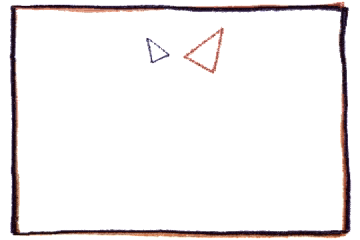
\includegraphics[scale=0.3]{sample65dance.png} & 
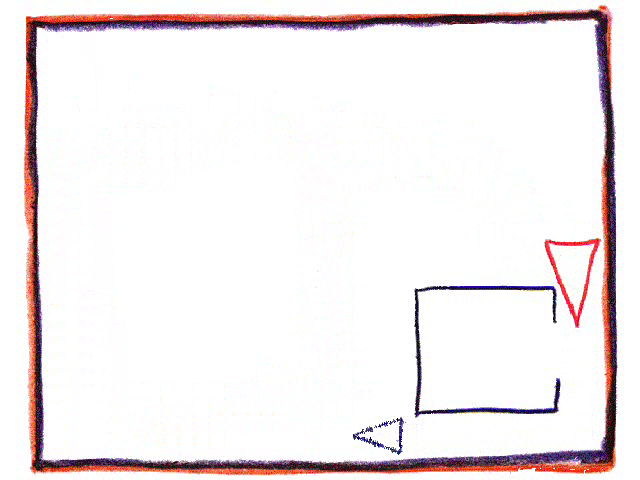
\includegraphics[scale=0.15]{sample174chase.png} &
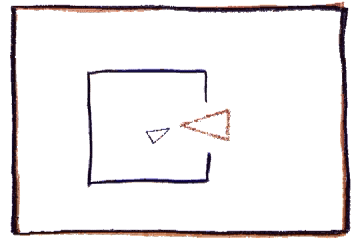
\includegraphics[scale=0.3]{sample198coax.png}
\end{tabular}
\label{tab:gt}
\caption{Stills from animations (a) Dancing Video, (b) Chase Video and (c) Coaxing Video }
\end{figure}

\section{Extracting Objects: }
We selected $4$ of the videos namely Coaxing and Chase to use in our project. In these videos there were three objects, a red triangle, a smaller blue triangle and and a rectangular box. In the rest of the two videos the rectangular box is absent.\\
The frames are converted to gray scale and following steps are done :\\
\\ \hspace*{10pt} In the first step, we determine the two triangles in the video and track them by background subtraction. To do so one frame of the video is taken as the base frame $frame_0$ and for all the images we calculate the difference of frames :
	$$difference_i = frame_i - frame_0$$
Then we apply erosion and dilation to remove the noise in the image. At this step the triangles are not separated from each other but they are separated from rest of the static objects in the video. We use various image processing techniques to separate the triangles which are described below.
\hspace*{10pt} The triangles are made of lines segments. Therefore the most obvious way of determining a triangle is to determine it's edges. Hough transform is a very effective way of identifying the line segments in a data.\\

\subsection{Separation of the triangles}
\hspace*{10pt} In the video the sizes of both the triangles are significantly different. We take the benefit of f this difference. The line segments corresponding to the bigger triangle will have high intensity in the $(R, \Theta)$ space compared to that of the smaller triangle.\\
\hspace*{10pt} We take top three peaks in the $(R, \Theta)$ space and get the points corresponding to them in $(X,Y)$ space. These points form the bigger triangle. Once the line of a single triangle has been extracted, we can easily get its vertices by calculating the intersection points of the lines.\\
\hspace*{10pt} After separating the larger triangle, we apply same Hough Transform technique in the remaining points to get the edges of the smaller triangle and vertices subsequently.\\

\begin{figure}[h]
\center
\begin{tabular}{cc}
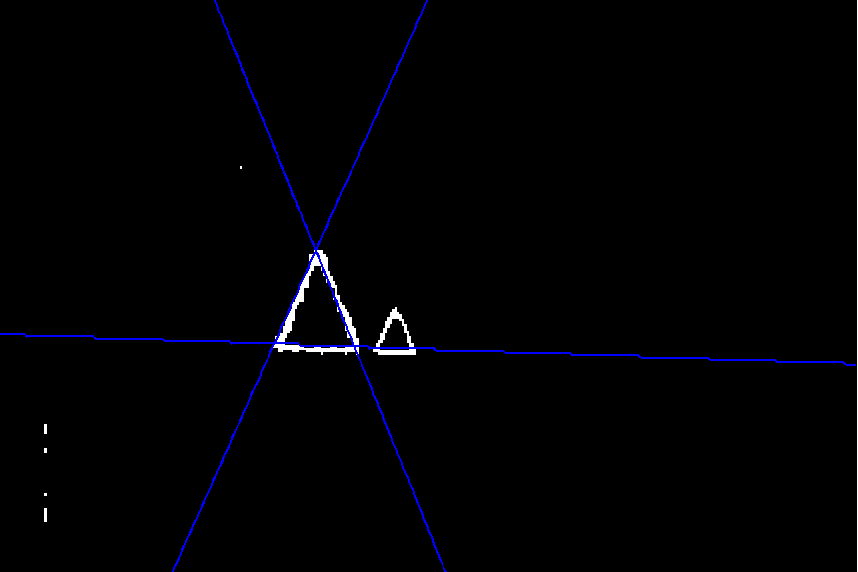
\includegraphics[scale=0.30]{0002l.png} & 
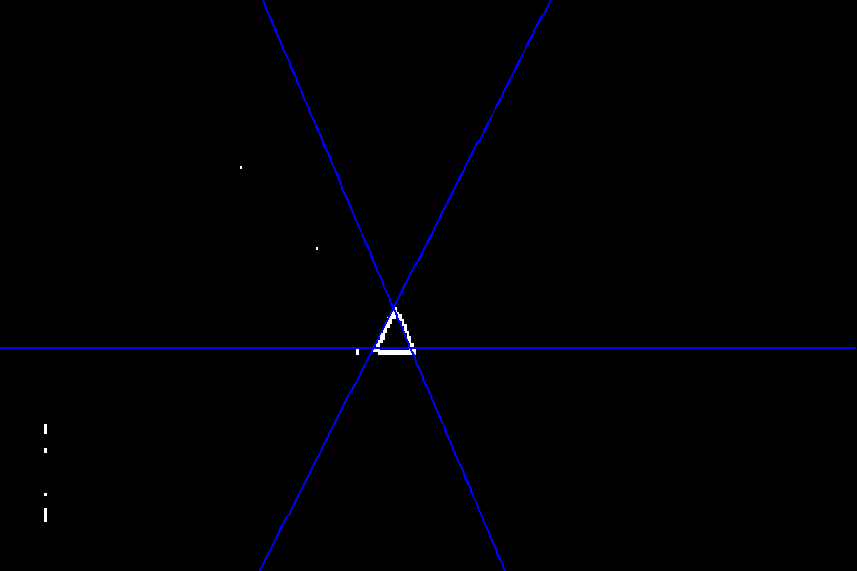
\includegraphics[scale=0.30]{0002s.png}
\end{tabular}
\label{tab:gt}
\caption{Two triangles as detected by Hough Transform}
\end{figure}

\subsection{Determination of the Rectangle }
Since the rectangle is static in the video. We can determine it in just one frame. After the triangles are identified and separated from the frame, we remove the white background and the black-red boundary. Then we are left with the points corresponding rectangle. On these points, applying hough transform, the four edges of the rectangle are determined. The four vertices of the rectangle are determined by intersection of the edges. And the vertices of the opening in the rectangle is determined by linear interpolation.\\
\begin{figure}[h]
\center
\begin{tabular}{c}
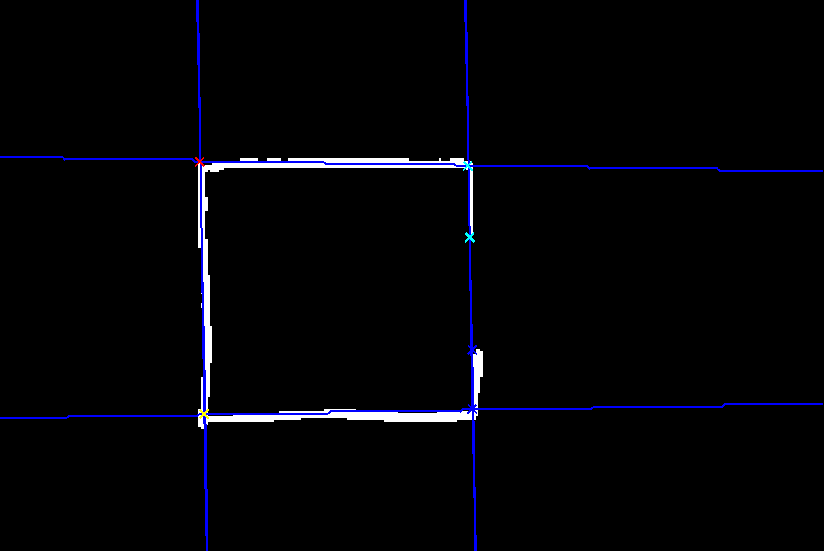
\includegraphics[scale=0.30]{rectCoax.png}
\end{tabular}
\label{tab:gt}
\caption{The detected rectangle and its vertices in Coaxing Video}
\end{figure}


\section{Feature Extraction}
 Feature extraction is one of the most important parts of this project. The actions in a image sequence are represented bye the motion of the objects in the video. Therefore the motion of the objects in the video is highly dependent on the other object. To discover actions in the video, we need to get the features which are relevant to their interaction and their individual actions.\\
 \hspace*{10pt} Let the feature vector of a frame is $F = \{f_1 , f_2, \cdots, f_n\}$. Here are the features which we calculated and used different subsets of these in further works :- \\

 \subsection{Position of the Triangles : }
The interaction between the objects is highly dependent on the position of the objects. The individual position of the objects also infer their relative positions.\\
\hspace*{10pt} In object identification, we calculated the coordinates of the vertices of the triangles. From them we calculate the coordinates of the centroid of each of the triangle which is also assumed to be the position of the triangle.

\subsection{Orientation of the Triangles : }
The extent of interaction between the triangles is dependent on their relative orientation, e.g. if both the triangles are facing each other(exactly opposite orientation), then they are more likely to interact or express an action.\\
\hspace*{10pt} The orientation of the triangle is calculated by tracking the motion of the triangle. The vertex relatively aligned in the direction of the motion with respect to the centroid of the triangle is the head of the triangle. The made by the line joining the centroid with the head of the triangle is the orientation of the triangle.

\begin{figure}[h]
\center
\begin{tabular}{c}
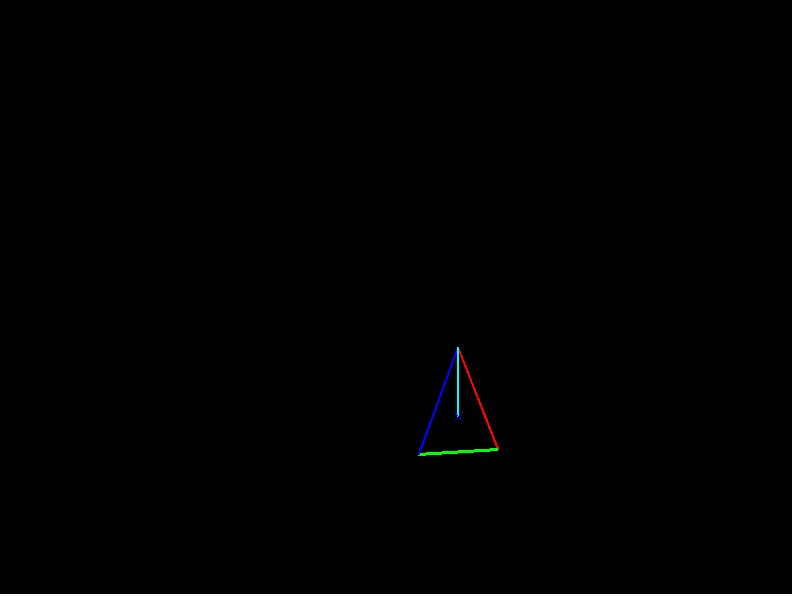
\includegraphics[scale=0.30]{orientation.png}
\end{tabular}
\label{tab:gt}
\caption{The detected rectangle and its vertices in Coaxing Video}
\end{figure}

\subsection{Visibility of the triangle :}
In the videos where the rectangular box is there, the fact that whether the two triangles are able to see each other or not and if they can then to what extent. Therefore we chose visibility too as a feature vector in the triangle.\\
\hspace*{10pt} The visibility of two triangle is a non-negative number $v \in [0, 1]$. Here $0$ means that the two triangles are completely occluded with the rectangle and $1$ means that they are completely visible to each other and any value between $0$ and $1$ is measure of extent they are visible.\\
\hspace*{10pt} The visibility of the triangles is calculated as follows :- \\
\hspace*{20pt} $1-$ Draw the supporting tangents for the two triangles. Now part of the rectangle which falls between these two lines is determined. We take the projection of this part of rectangle in directions of perpendicular to the  supported tangents is calculated. The fraction of this projection with total distance between supporting tangents is the measure of the visibility of the triangles. The figure below explains feature :- \\

\begin{figure}[h]
\center
\begin{tabular}{c}
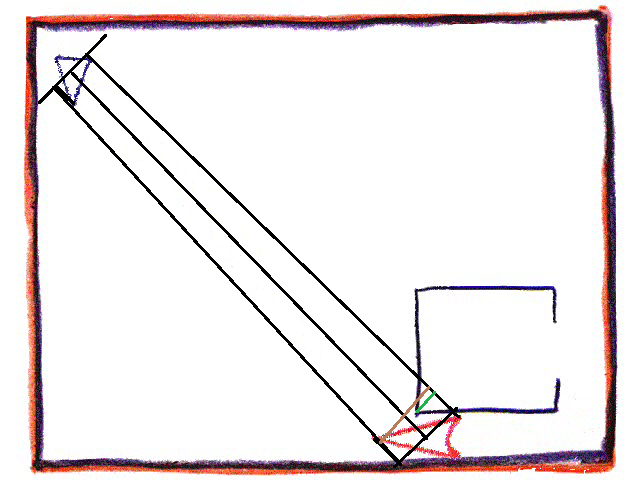
\includegraphics[scale=0.30]{visibility.png}
\end{tabular}
\label{tab:gt}
\caption{Visibility of triangles :  The brown line between the two supporting tangents is the distance between the lines and the green line is measure of occlusion and the ratio of lengths of green and brown lines is the measure of visibility}
\end{figure}

\subsection{Feature vector :}
The feature vector of a frame is a subset or derived of the previously calculated features. Let the centroid is represented by $C$ and orientation is represented by$\theta$ and the visibility between the triangles $t_1$ and $t_2$ is $v$. Then Following are some feature vector used :-\\

1- Ignore the visibility factor in both the triangles and take only the centroids and orientation of the triangles \\
\hspace*{20pt} $[C_{t_1}$ $C_{t_2}$ $\theta_1$ $\theta_2]$\\
2- Include the visibility factor with other features\\
\hspace*{20pt} $[C_{t_1}$ $C_{t_2}$ $\theta_1$ $\theta_2$ $v]$\\
3- Since $\theta$ is in $S_1$ topology, i.e it is periodic value with period $360$. It's values of $0$ and $360$ is overlapping. Therefore to remove this shortcoming, we can use the $sin$ and $cos$ of the $\theta$.\\
\hspace*{20pt} $[C_{t_1}$  $C_{t_2}$  $sin\theta_1$  $cos\theta_1$  $sin\theta_2$  $cos\theta_2]$\\

\section{Actions in the Visual Sequence :}
Actions in visual sequences are result of complicated motions of the objects in it. This complicated motion can be learnt by HMMs and appropriate feature vectors. We follow two approaches for learning the actions in the video. One is completely unsupervised hierarchical cluster based method and other is user labelled unsupervised method. These two methods differ on how we provide the input to the HMMs and how to use the created HMHs.\\

\colorbox{gray}{\Large \bf A. Completely Unsupervised Method} 

\subsection{Learning the HMM :}

\begin{minipage}{0.4\textwidth}
\begin{flushleft} \large
We break the whole video into frame sequences each having $N$ frames and each of sequences overlap by $M$ frames. The choice of $N$ and $M$ is dependent on the approximate length of the action sequences and the time interval in which the action appears. For each of these sequence we learn HMM on that.

\end{flushleft}
\end{minipage}
\begin{minipage}{0.4\textwidth}
\begin{flushright} \large

\center
\begin{tabular}{c}
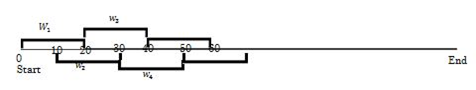
\includegraphics[scale=0.5]{interval.png}
\end{tabular}
\label{tab:gt}

\end{flushright}
\end{minipage}\\[3cm]

\subsection{Hierarchical Clustering :}
Once we get the HMMs on all the image sequences, we calculate the distance between these HMMs. Here we take the Mutual Acceptance as the distance between to HMM. Mutual acceptance is defined as :-\\

$$dist(S_1, S_2) = \frac{|logP(S_2|\lambda _ 1)|}{N_1} +\frac{|logP(S_1|\lambda _ 2)|}{N_2} $$
Where : \\
\hspace*{20pt} $\lambda_1$ and $\lambda_2$ are HMMs trained on data $S_1$ and $S_2$ respectively.\\
\hspace*{20pt} The length of $S_1$ is $N_1$ and that of $S_2$ is $N_2$.\\

Based on this measure a hierarchical clustering is created. We used in-built function of Matlab for such clustering. A hierarchical clustering is recursively merging of clusters or points to form a single cluster in the end. Thus we get tree in which different clusters are merged at different levels based on the distance measure provided and a merging method. We used Mutual acceptance as calculated above as the distance measure and 'ward' method for merging clusters.

\begin{figure}[h]
\center
\begin{tabular}{c}
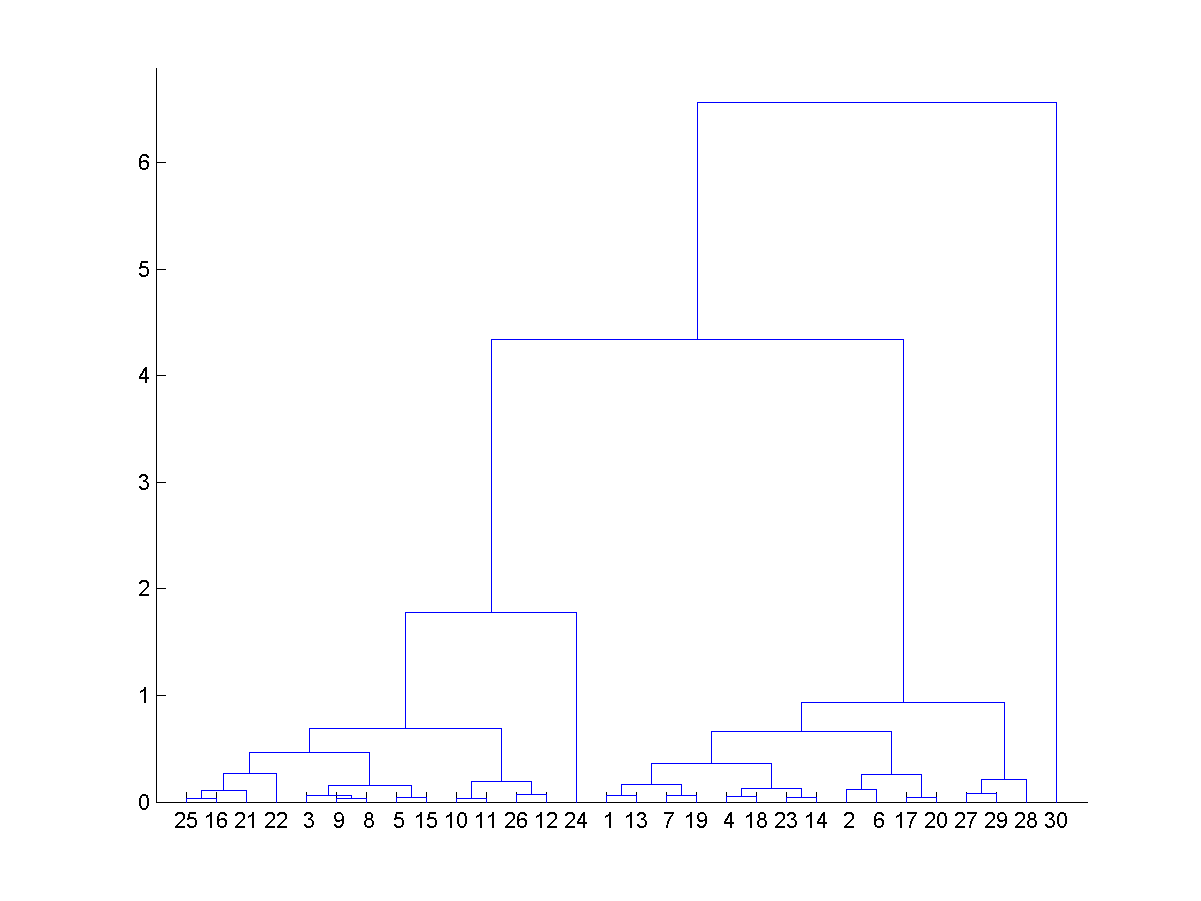
\includegraphics[scale=0.30]{dendoCoax.png}
\end{tabular}
\label{tab:gt}
\caption{The hierarchical clustering created for Coaxing video, top 30 nodes are shown}
\end{figure} 
 
 The leafs in the tree represent the individual points in the dataset while the internal nodes represent the clusters of points. The points merging near the leaves are more similar to points merging far from leaves. This hierarchical clustering helps us to classify the data into specific number of clusters. We just need to cut the tree at appropriate level for this.\\
 
 \colorbox{gray}{\Large \bf B. Used labelled Unsupervised Method}

\subsection{Labelling the actions :}
In the Coaxing video, there are 4-5 types of actions namely {\dn \7{G}\qq{m} {\rs ,\re} V\3C3w\qq{r} mArAn{\rs ,\re} K\?l{\rs ,\re} lr}. Here we label all the actions in the video manually. 
%\chapter{Language Association } 
 
 
 
 
 
%%%%%%%%%% APPENDIX %%%%%%%%%%
\appendix
\chapter{Hough Transform}
\hspace*{10pt} Given a point $(x, y)$ on a line $L$. If the distance of line from origin is $r$ and the normal to the line from origin makes $\theta$ angle from the positive $x-axis$ then, the equation of the line can be written as :-\\
$$r = x cos\theta + y sin\theta$$
For each point $(x,y)$ in the combined data of triangle we get the corresponding $(r, \theta)$ pairs for $\theta \in (-180, 180]$ at the intervals of $\theta _ 0$. In this way $(R, \Theta)$ space is created. In this space the local maxima correspond to line segments. Higher the intensity of the maxima, larger the line segment corresponding to the point.\\

\chapter{Hidden Markov Models}
Hidden Markov Models(HMM) are dynamic Bayesian network. HMM are modelled as certain number of hidden states and some visible state. All of these states have probabilistic dependencies and these probabilistic dependencies are the characteristics of a particular HMM. Mathematically, these are modelled as follows :-\\
$$\lambda = \{A, B, \pi \}$$
Where : 
\hspace*{20pt} $A :$ State Transition Probabilities 
\hspace*{20pt} $B :$ Observation Symbol Probabilities
\hspace*{20pt} $\pi :$ Initial Probability Distribution
Like all dynamic Bayesian networks, the value of a state in HMM depends on values of  previous $k$ states. In this project, we take $k$ as $1$. So here the value of a state depends only on the previous state

\section{Learning an HMM }
We initialise the probabilities of HMM with selective random values i.e $\pi$. Now given the data, these probabilities are learnt by iteration. The values of these probabilities after these iterations are the characteristics of the HMM of the data.

\section{Loglikelihood :}
Given a learnt HMM $\lambda $ on some data $S$, and given a test $S_0$ data we can measure the similarity of this data to the HMM. This value is represented as :- \\
$$logLik = log(P(S_0 | \lambda))$$
This value is used to measure the distances between two HMMs.\\
\section{Distances Between HMMs}
Let a HMM learnt on Data $S_1$ of length $T_1$ is $\lambda _1$ and that on data $S_2$ of length $T_2$ is $\lambda _ 2$. The distance between the HMMs is defined as :- \\

$$dist(S_1, S_2) = \frac{|logP(S_2|\lambda _ 1)|}{T_1} +\frac{|logP(S_1|\lambda _ 2)|}{T_2} $$
  

%%%%%%%%%% BIBLIOGRAPHY %%%%%%%%%%
\chapter*{Bibliography}
%
\begin{description}

\item Author, I. (Year). \emph{Book Title}, Publisher; Place of publication.

\item Lamport, L. (1986), \emph{\LaTeX: A Document Preparation System}, Addison-Wesley; Reading, MA.

\item Author, I. (Year). `Journal article title', \emph{Journal}, \textbf{Vol}, pp.first--last.

\item Smith, A.D.A.C. and Wand, M.P. (2008). `Streamlined variance calculations for semiparametric
mixed models', \emph{Statistics in Medicine}, \textbf{27}, pp.435--48.

\end{description}

\end{document}